% !TEX root = ../../seminar.tex

\subsection{Evaluate Process}
\label{subsec:evaluate process}

The last step of the process proposed here is to reflect on the process itself. After discussing the study and finishing it in the step before (see section \ref{subsec:discussion}), Dyb{\aa} \etal recommend to reflect on how well each step was performed and what could be improved in the next iteration. To support this they recommend using \emph{after-action reviews} (AAR) and \emph{postmortem analysis} (PMA) \cite{Dyba2005}.

AAR is a short meeting of 10 to 20 minutes answering the four questions in figure \ref{fig:aar_pma}, left box. This method can also be used at any other point the process when need is to reflect on or rethink the current situation\cite{Dyba2005}.

PMA is similar to AAR but with a deeper insight. Therefore it lasts for several hours up to a full day. It answers the questions in figure \ref{fig:aar_pma}, right box \cite{Dyba2005}. Here conclusions can be drawn to improve upcoming EBSE cycles and further research in general. This method can give insight issues like: which methods worked out as planned and which did not. Where was time lost and deadlines missed. Which technique proves to be used in upcoming studies. 

After this step the whole process starts over again with the next research question.

\begin{figure}
	\centering
	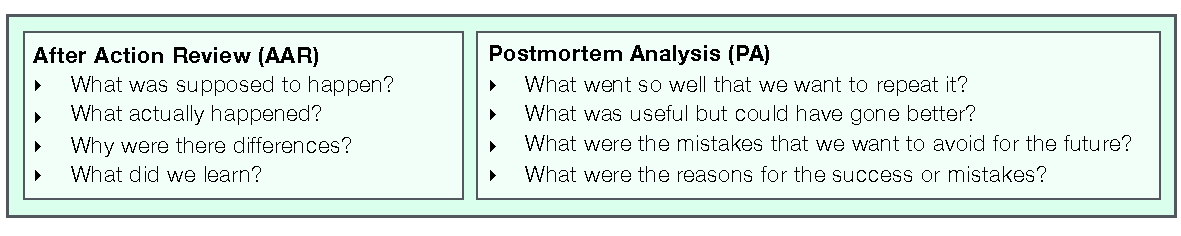
\includegraphics[width=12.5cm]{figures/aar_pma.pdf}
	\caption{\todo{text, sources}}
	\label{fig:aar_pma}
\end{figure}
